%% LyX 2.3.2 created this file.  For more info, see http://www.lyx.org/.
%% Do not edit unless you really know what you are doing.
\documentclass[10pt,twoside,twocolumn,british,english,UKenglish]{article}
\usepackage{mathptmx}
\usepackage[T1]{fontenc}
\usepackage[latin9]{inputenc}
\usepackage[letterpaper]{geometry}
\geometry{verbose,tmargin=3cm,bmargin=3cm,lmargin=1.5cm,rmargin=1.5cm,footskip=2cm,columnsep=1cm}
\usepackage{fancyhdr}
\pagestyle{fancy}
\setcounter{secnumdepth}{5}
\setcounter{tocdepth}{5}
\setlength{\parskip}{\medskipamount}
\setlength{\parindent}{0pt}
\usepackage{array}
\usepackage{refstyle}
\usepackage{textcomp}
\usepackage{amsmath}
\usepackage{amsthm}
\usepackage{graphicx}

\makeatletter

%%%%%%%%%%%%%%%%%%%%%%%%%%%%%% LyX specific LaTeX commands.

\AtBeginDocument{\providecommand\secref[1]{\ref{sec:#1}}}
\AtBeginDocument{\providecommand\subsecref[1]{\ref{subsec:#1}}}
\AtBeginDocument{\providecommand\tabref[1]{\ref{tab:#1}}}
\AtBeginDocument{\providecommand\parref[1]{\ref{par:#1}}}
\newcommand{\noun}[1]{\textsc{#1}}
%% Because html converters don't know tabularnewline
\providecommand{\tabularnewline}{\\}
\RS@ifundefined{subsecref}
  {\newref{subsec}{name = \RSsectxt}}
  {}
\RS@ifundefined{thmref}
  {\def\RSthmtxt{theorem~}\newref{thm}{name = \RSthmtxt}}
  {}
\RS@ifundefined{lemref}
  {\def\RSlemtxt{lemma~}\newref{lem}{name = \RSlemtxt}}
  {}


%%%%%%%%%%%%%%%%%%%%%%%%%%%%%% Textclass specific LaTeX commands.
\numberwithin{equation}{section}
\numberwithin{figure}{section}
\numberwithin{table}{section}

\@ifundefined{date}{}{\date{}}
%%%%%%%%%%%%%%%%%%%%%%%%%%%%%% User specified LaTeX commands.
%\usepackage{draftwatermark}
%\SetWatermarkText{\textsc{Prototype}}
%\SetWatermarkColor[rgb]{0.8,0.9,0.8 }
%\SetWatermarkFontSize{1cm}
%\SetWatermarkScale{5}
\usepackage[missing=Help!,notags={No tags?},dirty=dirty]{gitinfo2}

\PassOptionsToPackage{UKenglish}{babel}
\usepackage[UKenglish]{babel}% http://ctan.org/pkg/babel
\usepackage{fancyhdr}
\usepackage[UKenglish]{datetime}
\usepackage{lastpage}
\usepackage{lipsum}

\usepackage{hyperref}
\hypersetup{
plainpages    = true,
         breaklinks    = true,% not default in dvips mode, so we must specify
         hypertexnames = false,%not ideal, but needed when pagenums duplicate (`i' vs. `1')
         pageanchor    = true,
         pagecolor     = blue,
         anchorcolor   = blue,
         colorlinks    = true, %Colours links instead of ugly boxes
         urlcolor      = blue, %Colour for external hyperlinks
         linkcolor     = blue, %Colour of internal links
         citecolor     = red %Colour of citations
}

\fancyhf{}

\renewcommand{\headrulewidth}{1pt}
\renewcommand{\footrulewidth}{1pt}

\fancyhead[C]{1839 English Rules}
\fancyhead[LE,RO]{\textit{ \nouppercase{\leftmark}} }
\fancyhead[LO,RE]{\textit{ \nouppercase{\rightmark}} }

\fancyfoot[LE,RO]{ Version: \gitFirstTagDescribe}
\fancyfoot[LO,RE]{ Date: \gitCommitterDate}

\fancyfoot[C]{Page: \thepage\  of  \pageref{LastPage}}

\pagestyle{fancy}

\makeatother

\usepackage{babel}
\begin{document}
\author{\noun{1839}\\
\noun{English Rules}\\
\noun{Game design: J C Lawrence}}
\title{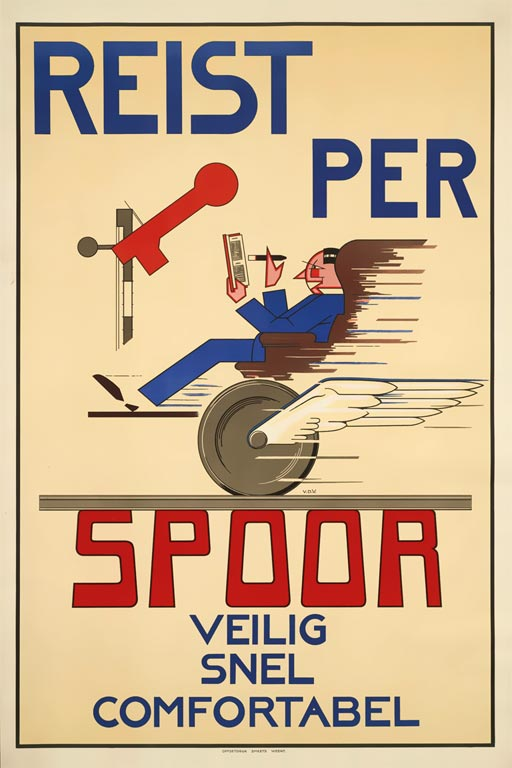
\includegraphics[height=7in]{masthead}}

\maketitle
\emph{``Travels safely by rail quickly and comfortably'' - }promotional
poster probably from 1932 by Nicolaas van de Vecht\emph{.}

\tableofcontents{}

\clearpage{}

\part{Overview\label{par:Overview}}

\section{Introduction\label{sec:Introduction}}

Waffly mumble mumble words about theme and history that conceivably
might related to the game here.

The player with the largest net worth at the end of the game wins
(see \secref{Game-End}).

\section{Components\label{sec:Components}}
\begin{itemize}
\item 1 set of game rules (this document).
\item 1 game map.
\item 1 stock market (also contains the round track).
\item 1 IPO and Bank Pool chart \emph{(currently not provided)}.
\item Many track tiles (yellow, green, brown and gray).
\item Trains (5 yellow, 6 green, 6 blue, 5 light brown, 5 dark brown, 5
red, 3 gray, 8 purple).
\item 2 sets of 4 player number cards numbered 1 through 4 (one set blue
\& one set red).
\item For each of 16 public companies:
\begin{itemize}
\item Public company charter.
\item 9 share certificates:
\begin{itemize}
\item One 20\% director's share certificate.
\item Eight 10\% share certificates.
\end{itemize}
\item 5 station markers.
\item 1 stock price marker
\end{itemize}
\item 12 private companies (2 green, 5 blue, 5 brown, 4 red).
\item 32 government station markers \emph{(not count-limited)}.
\item 1 round marker.
\item \textasciitilde\foreignlanguage{british}{\textflorin }20,000 in
money \emph{(not provided)}.
\end{itemize}

\section{Etiquette\label{sec:Etiquette}}
\begin{itemize}
\item To help the game progress smoothly, each player should consider their
upcoming choices while other players are taking their turns.
\item Use of paper, pencils/pens, calculators and similar aids is recommended
to assist players in making timely and accurate decisions.
\item Players should act simultaneously when doing so would not otherwise
affect the game, such as when operating public companies whose choices
do not affect each other.
\end{itemize}

\part{Rules\label{part:Rules}}

\section{Setup\label{sec:Game-Setup}}
\begin{itemize}
\item Place the map, Stock Market, public company charters, shares and track
tiles where they can be easily seen and accessed.
\item Pick otherwise unused areas around the board to serve as the IPO and
Bank Pool\emph{ (components not provided at this time).}
\item Place the round marker on the ``SR'' space on the round track on
the Stock Market.
\item (\emph{2-player game only}) Discard the following from the game:
\begin{itemize}
\item \#3 and \#4 player number cards of both colours.
\item \noun{Nederlandsche Fabriek van Werktuigen en Spoorwegmaterieel} blue
private company.
\item \noun{Cr�dit Mobilier }blue private company.
\item \noun{Lodewijk Pincoffs} brown private company.
\item \noun{Ketwich \& Voombergh }brown private company.
\end{itemize}
\item (\emph{3-player games only}) Discard the following from the game:
\begin{itemize}
\item \#4 player number cards of both colours.
\item \noun{Cr�dit Mobilier }blue private company.
\item \noun{Ketwich \& Voombergh }brown private company.
\end{itemize}
\item Place 3 ``SAVED'' markers with the \noun{Nederlandsche Fabriek van
Werktuigen en Spoorwegmaterieel} blue private company.
\item Randomly assign a 20\% director's share certificate of a founding
public company (see \subsecref{Public-Company-Overview}) and a matching
10\% share certificate to each of the brown private companies remaining
in the game.
\item Assign two 10\% share certificates of the public company assigned
to the \noun{Rijkswaterstaat} brown private company to the \noun{Schielands
Hoge Zeedijk} blue private company.
\item Place \textflorin 80 in discounts from the bank on each of the blue
private companies other than the \noun{Schielands Hoge Zeedijk} blue
private company.
\item Place \textflorin 40 in discounts from the bank on the \noun{Schielands
Hoge Zeedijk} blue private company.
\item Place the private companies with their accompanying tokens, share
assignments and discounts where they can be easily examined by all
players.
\item Separate the player number cards by colour, set one colour aside and
randomly assign the remaining player number cards, one card per player.
\item Give each player \foreignlanguage{british}{money:}
\begin{itemize}
\item 2-players: \textflorin 740
\item 3-players: \textflorin 660
\item 4-players: \textflorin 580
\end{itemize}
\end{itemize}
\begin{table*}
\begin{description}
\item [{%
\begin{tabular}{>{\centering}m{0.6in}>{\centering}m{2cm}>{\centering}m{1in}>{\centering}m{0.6in}>{\centering}m{0.5in}>{\centering}m{0.8in}>{\centering}m{0.8in}>{\centering}m{0.8in}}
Phase & Train Type & Quantity & Price & Train Limit & Track Tiles Available & Trains Rusted & Operating Rounds per Set\tabularnewline
\hline 
\hline 
Yellow & L2\\
2 & Unlimited\\
5 & N/A\\
\textflorin 80 & 4 & Yellow &  & 1\tabularnewline
\hline 
Green & L2+1 \\
3+ & Unlimited\\
6 & N/A\\
\textflorin 160 & 4 & Yellow\\
Green &  & 2\tabularnewline
\hline 
Blue & L2+\\
5+ & Unlimited\\
6 & N/A \textflorin 250 & 4 & Yellow\\
Green & Yellow & 2\tabularnewline
\hline 
Light Brown & R4 & 5 & \textflorin 400 & 4 & Yellow\\
Green\\
Brown & Green & 3\tabularnewline
\hline 
Dark Brown & 7 & 5 & \textflorin 450 & 3 & Yellow\\
Green\\
Brown & Blue & 3\tabularnewline
\hline 
Red & R2+ & 5 & \textflorin 500 & 2 & Yellow\\
Green\\
Brown & Light brown & 3\tabularnewline
\hline 
Gray & 4 & 3 & \textflorin 700 & 2 & Yellow\\
Green\\
Brown\\
Gray & Dark brown & 4\tabularnewline
\hline 
Purple & Diesel & Unlimited\\
(10 are supplied\} & \textflorin 900 & 2 & Yellow\\
Green\\
Brown\\
Gray & Red & 4\tabularnewline
\hline 
\end{tabular}}]~
\end{description}
\centering{}\caption{Game Phases\label{tab:Game-Phases}}
\end{table*}


\section{Game Overview \label{sec:game-overview}}
\begin{itemize}
\item 1839 begins with the auction of the private companies (see \secref{Private-Auction}).
\item After auctioning the private companies, the game consists of an alternating
series of Stock Rounds and sets of one to four Operating Rounds\noun{.
}The round marker is used to track the game's progress through the
rounds.
\item In Stock Rounds, players may buy and sell shares of public companies,
take and lose directorship of public companies (see \secref{Companies})
and float new public companies (see \secref{Stock-Rounds}). 
\begin{itemize}
\item At the end of each Stock Round, the player order for the next Stock
Round is determined by the order in which the players cease acting
(see \subsecref{Stock-Round-overview}).
\item The number of Operating Rounds per set after a Stock Round\noun{ }is
determined by the current game phase at the end of the Stock Round
(see \tabref{Game-Phases} \& \secref{Game-Phases})\noun{.}
\end{itemize}
\item In Operating Rounds\noun{,} public companies are operated by their
directors: buying private companies from players, building track and
stations, running and buying trains, withholding or paying dividends
to shareholders, and being nationalised (see \secref{Operating-Rounds}
\& \subsecref{Public-company-nationalisation} \& \subsecref{Public-company-nationalisation}).
\begin{itemize}
\item Public companies on the Major Stock Market act in Operating Rounds,
before public companies on the Local Stock Market. Public companies
in each market act in descending order of their stock prices (see
\subsecref{company-operating-order}).
\end{itemize}
\item The game starts in\noun{ }yellow phase with the yellow trains (see
\tabref{Game-Phases} \& \secref{Game-Phases}).
\begin{itemize}
\item Game phases are tied to their matching train colours (see \tabref{Game-Phases})
and change immediately when the first train of a new colour is bought
by a public company. 
\item Additional par prices, track tile types and other changes accompany
some game phase changes (see \secref{Game-Phases}).
\end{itemize}
\item An alternating sequence of Stock Rounds\noun{ }and sets of Operating
Rounds\noun{ }continues until the end of the game (a player is agreed
to have won, a player bankrupts, a stock price reaches \textflorin 500,
or a complete set of Operating Rounds is finished in purple phase)
(see \secref{Game-End}).
\item The player with the largest net worth at the end of the game wins
(see \secref{Game-End}).
\item The holdings of players, public companies and systems are public information
and must be clearly displayed and visible to all players at all times.
\end{itemize}

\section{Private Auction \label{sec:Private-Auction}}
\begin{itemize}
\item The private auction starts with the player with the \#1 player number
card and proceeds in rotating player number card order, with the \#1
player number card following the largest player number card.
\item On their turn each player must either do both the following or either
of the following twice:
\begin{itemize}
\item Purchase one of the remaining private companies at its current price,
paying that price to the bank (face value minus any discounts already
on the private company) and discarding any discounts on that private
company to the bank (see \subsecref{Private-Companies}).
\begin{description}
\item [{Exception:}] The active player cannot purchase a private company
that they have discounted on that turn.
\end{description}
\end{itemize}
or:
\begin{itemize}
\item Discount one of the remaining private companies by \textflorin 20
by placing \textflorin 20 from the bank on the private company.
\begin{description}
\item [{Exception:}] The active player cannot discount a remaining private
company if:
\begin{itemize}
\item One of the remaining private companies had a current price of zero
or below before the active player's turn (face value minus any discounts
already on the private company). In this case the private company
is purchased at no cost.
\end{itemize}
or:
\begin{itemize}
\item (\emph{3 \& 4 player games only}) None of the other players could
afford any of the remaining private companies at the start of the
active player's turn, and the active player can afford one or more
of the remaining private companies that they have not discounted on
that turn.
\end{itemize}
or:
\begin{itemize}
\item (\emph{2-player games only}) None of the other players could afford
any of the remaining private companies at the start of the active
player's turn, and the active player can afford one or more of the
remaining private companies that they have not discounted on that
turn and they have not purchased a private company on this turn.
\end{itemize}
\end{description}
\end{itemize}
\item Player purchases are limited to their available cash.
\item When a brown private company is purchased, the assigned Founding Public
Company must immediately be parred on the Major Stock Market (see
\subsecref{Stock-Market-Overview}).
\item When all private companies have been purchased, the private auction
ends:
\begin{itemize}
\item The Stock Round starts with the next player in rotating player number
card order.
\end{itemize}
\end{itemize}

\section{Stock Rounds\label{sec:Stock-Rounds}}

\subsection{Stock Round overview \label{subsec:Stock-Round-overview}}
\begin{itemize}
\item Stock Rounds start with the player with the \#1 player number card
and proceed in rotating player number card order with the \#1 player
number card following the largest player number card.
\begin{description}
\item [{Exception:}] The first Stock Round after the private auction starts
with the next player in rotating player number card order (see \secref{Private-Auction}).
\end{description}
\item On their turn a player may pass or do any or all of the following
in the following order:
\begin{itemize}
\item Sell shares of one or more public companies (see \subsecref{Selling-shares}).
\item One of:
\begin{itemize}
\item Buy a single stock certificate from the Bank Pool, IPO or a company
treasury (see \subsecref{Buying-shares}).
\end{itemize}
Or:
\begin{itemize}
\item Have one of the companies they direct redeem one or more of its shares
from the Bank Pool (see \subsecref{Redeeming-shares}).
\end{itemize}
\item Sell shares of one or more public companies (see \subsecref{Selling-shares}).
\end{itemize}
\item Player purchases are limited to their available cash.
\item If a player passes, they may act in the Stock Round on their next
or a later turn.
\item When players pass in the Stock Round, they take the lowest numbered
available player number card of the other colour.
\item When players act instead of passing in the Stock Round, they return
any player number card of the other colour that they have to the supply.
\begin{itemize}
\item The player with the next larger number card of the other colour then
swaps their card for the returned card, repeating as necessary for
the other players such that the other player number cards show the
order in which those players passed and ceased acting in the Stock
Round.
\end{itemize}
\item The Stock Round ends immediately when all the player number cards
of the other colour have been taken (all players have consecutively
passed).
\begin{itemize}
\item The player number cards of the current colour are returned to the
supply.
\item The player number cards of the other colour will determine the player
order in the next Stock Round.
\end{itemize}
\item At the end of each Stock Round the stock prices of floated public
companies with:
\begin{itemize}
\item No shares in the IPO or Bank Pool are moved right on the Stock Market
in operating order (see \subsecref{company-operating-order} \& \subsecref{Stock-price-movement}).
\item Shares in the Bank Pool are moved left on the Stock Market in operating
order (see \subsecref{company-operating-order} \& \subsecref{Stock-price-movement}).
\end{itemize}
\item The number of Operating Rounds in the ``set'' following the Stock
Round is controlled by the current game phase (see \secref{Game-Phases}).
\end{itemize}

\subsection{Selling shares\label{subsec:Selling-shares}}
\begin{itemize}
\item Players can sell shares that they own:
\begin{itemize}
\item That are not a director's certificate (see \subsecref{Company-directors}).
\item In Stock Rounds other than the first Stock Round following the private
auction.
\item Of public companies that have been parred (see \subsecref{Starting-or-floating}).
\end{itemize}
\item The sale price for sold shares for public companies floated in an
earlier Stock Round is the current stock price per share. Otherwise
the sale price is the stock price next to the left from the current
stock price on that Stock Market, or if already at the left end of
that market, the current stock price.
\item The sale process:
\begin{enumerate}
\item The selling player announces the shares they will be selling (which
public companies and the share counts being sold) and receives the
sale price of the share(s) in cash from the bank.
\item For each public company in operating order (see \subsecref{company-operating-order})
whose shares are sold, either:
\begin{itemize}
\item The director of that company (may be the same player) can have the
public company redeem all the shares being sold (see \subsecref{Redeeming-shares}).
\begin{itemize}
\item The company must have been floated, must have sufficient treasury
to pay for all the shares of the company being sold and must redeem
all the shares being sold at that time.
\end{itemize}
\end{itemize}
or:
\begin{itemize}
\item The stock price marker is moved left one space for each share sold
of that public company and the sold shares are placed in the Bank
Pool.
\begin{itemize}
\item If the stock price reaches the lowest price of that Stock Market,
it isn't moved further (see \secref{Stock-Market}).
\item If shares from multiple public companies are sold and their stock
prices end in the same space on the Stock Market, the selling player
must choose their relative order at that stock price, and they are
placed below any stock markers already at that location.
\end{itemize}
\end{itemize}
\end{enumerate}
\end{itemize}

\subsection{Buying shares\label{subsec:Buying-shares}}
\begin{itemize}
\item Shares may be bought from the IPO, Bank Pool and company treasury.
\begin{itemize}
\item Shares cannot be bought from a public company's treasury if shares
of that public company remain in the IPO.
\end{itemize}
\item Only one stock certificate can be bought per player-turn or action
in the Stock Round.
\item A player cannot buy a certificate of a public company if they already
hold 60\% of that company.
\item The first available certificate of a public company is always the
director's certificate (2 shares, 20\%, one certificate - see \subsecref{Starting-or-floating}
\& \subsecref{Company-directors}).
\item Players can buy non-director's certificates of public companies only
if they have been parred (see \subsecref{Starting-or-floating}).
\item A player cannot buy a certificate of a public company if they have
sold any shares of that company in the current Stock Round.
\begin{itemize}
\item They may buy certificates of that public company in future Stock Rounds.
\end{itemize}
\item The purchase price for share certificates is the number of shares
represented by the certificate, multiplied by the current stock price
of that company.
\item The purchase price is paid to the bank for shares bought from the
IPO or Bank Pool and to that company treasury for shares bought from
a company treasury.
\end{itemize}

\subsection{Redeeming shares \label{subsec:Redeeming-shares}}
\begin{itemize}
\item When a player sells shares during a Stock Round or Operating Round
(see \ref{subsec:Selling-shares} \& \ref{subsec:Emergency-train-buying}),
the public companies whose shares were sold may redeem those shares:
\begin{itemize}
\item The purchase is made before the stock price is changed due to the
stock sales.
\item The public company pays the current stock price from its treasury
to the bank for each of its sold shares and places the purchased shares
in its treasury.
\item The public company must have sufficient funds for and must redeem
all the shares of the company sold at that time.
\item This is not an action for the director of the company (see \subsecref{Stock-Round-overview}).
\end{itemize}
\item On a player's turn during a Stock Round, a company they direct can
buy any or all of its own shares from the Bank Pool.
\begin{itemize}
\item The public company pays the current stock price from its treasury
to the bank for each share bought and places them in its treasury.
\item This is an action for the director of the company in the Stock Round
(see \subsecref{Stock-Round-overview}).
\end{itemize}
\end{itemize}

\subsection{``Floating'' a public company\label{subsec:Starting-or-floating}}
\begin{itemize}
\item The first available share certificate of a public company is always
the director's certificate (2 shares, 20\%, one certificate).
\item The director's certificate of a public company can be bought from
the IPO by:
\begin{enumerate}
\item Placing all of the public company's shares in the IPO.
\item Selecting a par price on the Local or Major Stock Market and putting
the public company's stock price marker in the matching box on that
market, underneath any other markers already there (see \secref{Stock-Market}).
\begin{itemize}
\item Founding public companies that haven't previously been nationalised
must be parred on the Major Stock Market. If they have been nationalised
they can be parred as either Local or Major Public Companies (see
\subsecref{Public-Company-Overview}).
\end{itemize}
\item Paying twice that value to the bank and taking the director's share
certificate.
\item (\emph{If the public company is not a founding public company}) Reserve
two home station hexagons:
\begin{itemize}
\item Both hexagons must have a currently available and unreserved location
for a station marker.
\item No more than one of the two hexagons can be an OO hexagon or be a
big city (Amsterdam, Breda, Haarlem, Rotterdamn, or Utrecht, see \secref{Map-Explanation}).
\item Mark both hexagons with that public company's station marker placed
near but not in an available city circle.
\end{itemize}
\end{enumerate}
\item After the 20\% director's certificate of a public company has been
parred and bought, the remaining shares of the public company are
available for purchase in subsequent turns.
\item A public company is ``floated'' when no more than 40\% of the public
company's shares remain in the IPO:
\begin{itemize}
\item Station markers (see \tabref{Public-Companies}) are placed on the
company's charter. If the public company is not a founding public
company, two of the company's station markers will be marking hexagons
reserved for its home stations.
\item Money equal to 10 times the public company's current stock price price
is placed on the company's charter.
\begin{itemize}
\item (\emph{If the public company is not a founding public company}) The
company pays a fee to the bank equal to double the revenue of the
two home station hexagons.
\begin{itemize}
\item If the hexagon doesn't yet have a revenue, then the revenue of a yellow
track tile for that location is used.
\end{itemize}
\end{itemize}
\item The charter and control of the public company is given to the player
holding the director's certificate (see \subsecref{Company-directors}).
\end{itemize}
\end{itemize}

\section{Operating Rounds\label{sec:Operating-Rounds}}

\subsection{Operating Round overview \label{subsec:Operating-round-General}}
\begin{enumerate}
\item Private companies pay their revenue (shown on their certificate) from
the bank to their player or public company owners. Green, blue and
brown private companies pay their owners first, then red private companies
pay the bank (see \subsecref{Private-Companies}\& \subsecref{Red-private-companies}).
\item All floated public companies operate in operating order (see \subsecref{company-operating-order}).
\end{enumerate}

\subsubsection{Paying red private companies \label{subsec:Paying-red-private}}
\begin{itemize}
\item If there are multiple red private private companies in play, first
those owned by public companies are paid in company operating order
(see \subsecref{company-operating-order}) then player-owned red private
companies in player number card order.
\item If the owning public company has insufficient funds, then the public
company must sell shares from its treasury to raise the funds. Normal
share-selling rules apply (see \subsecref{Selling-shares}).
\begin{itemize}
\item If that is still not enough, the director must cover the arrears.
\end{itemize}
\item If the owning player's or director's cash is insufficient to cover
the arrears, the player must sell shares as needed to raise the funds.
Normal share-selling rules apply (see \subsecref{Selling-shares}).
\begin{itemize}
\item Public companies other than the company owning the red private company
being paid may redeem shares as they are sold for each red private
company's arrears (see \subsecref{Redeeming-shares}).
\item Stock prices are adjusted for stock sales after all red private companies
have been paid.
\item Director control of the public company that owns the red private company
being paid cannot be transferred to another player while raising funds
to pay the bank for that red private company (see \subsecref{Company-directors}).
\item The player cannot sell additional shares once enough money has been
raised to cover the arrears.
\end{itemize}
\item If the player is unable raise enough money to cover the arrears after
the public company has sold all the shares from its treasury, and
the player having contributed all possible funds and sold all shares
that can be legally sold (see \subsecref{Selling-shares}), then the
player is declared bankrupt (see \secref{Player-Bankruptcy}).
\item A public company that pays for a red private company with a director's
contribution necessarily ends its operations with no money in its
treasury.
\end{itemize}

\subsection{Operating order\label{subsec:company-operating-order}}
\begin{itemize}
\item Floated public companies (see \secref{Companies}) operate in order:
\begin{itemize}
\item First all the floated companies on the Major Stock Market in descending
order of stock prices, then all the floated companies on the Local
Stock Market in descending order of stock prices.
\item The stock price markers of public companies in the same space of the
Stock Market are stacked to indicate the order in which they'll operate,
from the top down.
\end{itemize}
\item As public companies operate, their stock price markers are turned
upside-down and moved to their new stock price location (see \subsecref{Stock-price-movement}):
\begin{itemize}
\item Stock price markers moving to the same space as other stock price
markers are placed under other face-up stock price markers and on
top of other face-down stock price markers (see \subsecref{Stock-price-movement}).
\end{itemize}
\item At the end of the Operating Round the upside-down stock price markers
are turned face-up so that the bottom face-down marker becomes the
top face-up marker. The result is that public companies sharing a
space in the stock price chart operate in the order in which their
share markers arrived at that space.
\item Each public company completes all of its actions in the Operating
Round before the next public company operates.
\end{itemize}

\subsection{Operating Round actions\label{subsec:Operating-round-actions}}
\begin{itemize}
\item Public companies perform the following steps in order:
\begin{enumerate}
\item (\emph{If the first time the public company is operat}ing) Place the
company's home station marker(s) on its home station location(s) (see
\subsecref{Starting-or-floating} \& \tabref{Public-Companies}).
\item \emph{(Optional)} Build track (see \subsecref{Build-track}).
\item \emph{(Optional)} Place or swap a station marker (see \subsecref{Place-station-marker}).
\item Run train(s) (see \subsecref{Run-train(s)}).
\item Pay or withhold dividends (see \subsecref{Pay-or-withhold}).
\item \emph{(May be optional)} Buy train(s) (see \subsecref{Buy-train(s)}
\& \subsecref{Emergency-train-buying}).
\end{enumerate}
\item (\emph{In green and later phases}) public companies may buy green
private companies from players at any time during the company's operation
for between \textflorin 1 and the face value of the private company
(see \subsecref{Private-Companies}).
\item (\emph{In blue and later phases}) public companies may buy blue private
companies from players at any time during the company's operation
for between \textflorin 1 and the face value of the private company
(see \subsecref{Private-Companies}).
\item The next public company in operating order (see \subsecref{company-operating-order})
then operates (see \subsecref{company-operating-order}), or if it
was the last public company in operating order, the Operating Round
ends (see \secref{game-overview}).
\end{itemize}

\subsubsection{Build track\label{subsec:Build-track}}
\begin{itemize}
\item A public company may place a yellow track tile or \emph{(green phase
or later)} upgrade one track tile or hexagon, and may place or upgrade
a different track tile or hexagon for a fee of \textflorin 20 paid
to the bank from the company treasury, both in addition to any terrain
or upgrade costs (see \subsecref{Track-placement-=000026-upgrades}
\& \subsecref{Upgrading-track} \& \secref{Game-Phases}). A public
cannot upgrade two track tiles or hexagons in the same Operating Round.
\begin{description}
\item [{Exception:}] A public company that owns the \noun{Het Laantje van
der Gaag} green private company (see \parref{Het-Laantje-van}) may
place an additional yellow track tile for a cost of \textflorin 20
paid to the bank in addition to any terrain or upgrade costs, from
the company treasury, closing the private.
\end{description}
\item Track placement and upgrade and terrain costs are paid from the public
company treasury to the bank.
\item Some hexagons are blocked and may not have track placed there until
their matching private companies have closed or been bought by a public
company (see \subsecref{Private-Companies-Overview}).
\end{itemize}

\subsubsection{Place or swap station marker(s) \label{subsec:Place-station-marker}}

\paragraph{Station marker overview\label{par:Station-marker-overview}}
\begin{itemize}
\item A public company cannot place:
\begin{itemize}
\item More or place than one station marker, not counting its home station(s),
per Operating Round. A private company special power cannot be used
by a public company to place a second station marker in an Operating
Round (see \subsecref{Saleable-private-companies}).
\item More than one station marker in the same hexagon.
\begin{description}
\item [{Exception:}] A public company that owns the \noun{Kabinet-Rochussen}
blue private company can move a station marker to a hexagon that already
has one of the company's station markers (see \parref{Kabinet-Rochussen}).
\end{description}
\item A station marker in the last available city circle of a hexagon that
is also the home station of a public company, if that company has
not already operated and placed its home station.
\end{itemize}
\end{itemize}

\paragraph{Place a station marker\label{par:Place-a-station}}
\begin{itemize}
\item In order to place a station marker, the public company must:
\begin{enumerate}
\item Have a station marker available to be placed (see \tabref{Public-Companies}).
\item Place a station marker in an empty city circle that can trace a single
continuous line of track to a previously placed station marker of
that company:
\begin{itemize}
\item Without passing through a city all of whose station-marker spaces
are filled with other companies' station markers and/or (major public
companies only) government station markers.
\item Crossing any hexagon-edge twice.
\end{itemize}
\item Pay a fee to the bank equal to the revenue of the location of the
newly placed station marker multiplied by the number of station markers
that company will have on the map after the placement.
\begin{itemize}
\item If the destination hexagon has no marked revenue, then use the revenue
of a legal yellow track tile for that hexagon.
\end{itemize}
\end{enumerate}
\end{itemize}

\paragraph{Swap station markers\label{par:Swap-station-markers}}
\begin{itemize}
\item To swap station markers, the public company must:
\begin{enumerate}
\item Have more than one station marker placed on the map.
\item Select one of its placed station markers and a placed station marker
of another public company.
\begin{itemize}
\item Both public company directors must agree to the swap.
\end{itemize}
\item Swap the locations of the two station markers.
\item Pay a fee to the bank equal to the revenue of the location the acting
company's station marker moved to, multiplied by the number of station
markers that company will have on the map after the move.
\begin{itemize}
\item If the destination location has no marked revenue, then use the revenue
of a legal yellow track tile for that hexagon.
\end{itemize}
\end{enumerate}
\end{itemize}

\subsubsection{Run train(s)\label{subsec:Run-train(s)}}
\begin{itemize}
\item A public company's income or revenue is the sum of the revenues of
all the trains the company owns during this step (see \secref{Trains-and-Running-Trains}).
\begin{itemize}
\item If a player indicates a route or routes that produces a higher total
revenue for the company, the director must use it.
\end{itemize}
\end{itemize}

\subsubsection{Pay or withhold dividends\label{subsec:Pay-or-withhold}}
\begin{itemize}
\item The director of a public company decides if the company's total revenue
is paid out in dividends to its shareholders or withheld in the company's
treasury , or a half-dividend is paid.
\item If the revenue is paid out in dividends:
\begin{itemize}
\item Each player receives as dividends from the bank the percentage of
the total revenue that corresponds to the total percentage of the
company shares they own.
\item Shares in the Bank Pool pay their fraction of the total revenue as
a dividend from the bank to the company treasury.
\item Shares in the treasury of a public company pay their dividend to the
system's treasury (see ).
\item No dividend is paid for shares in the IPO.
\end{itemize}
\item If the revenue is withheld:
\begin{itemize}
\item The entire revenue is paid from the bank to the company treasury.
\end{itemize}
\item If a half-dividend is paid:
\begin{itemize}
\item Half of the total revenue is paid from the bank to the company treasury.
\item Each player receives as dividends from the bank the percentage of
half the total revenue (rounding up) that corresponds to the total
percentage of the company shares they own.
\item Shares in the Bank Pool pay their fraction of half the total revenue
(rounding down) as a dividend from the bank to the company treasury.
\item Shares in the treasury of a public company pay their fraction of half
the total revenue (rounding down) from the bank to the company treasury.
\item No dividend is paid for shares in the IPO.
\end{itemize}
\item Paying or withholding dividends affects the company's stock price
(see \subsecref{Stock-price-movement}).
\end{itemize}

\subsubsection{Buy train(s)\label{subsec:Buy-train(s)}}

\paragraph{Train buying\label{par:Train-purchasing}}
\begin{itemize}
\item A public company that has not reached its train limit may buy trains
that would not cause it to exceed the train limit before any game
phase change caused by the purchase takes effect (see \secref{Game-Phases}
\& \subsecref{Train-Limit}).
\item Trains can be bought from the supply for face value, or from another
public company for any price agreed upon by the directors of both
companies (minimum \textflorin 1, also see \subsecref{Emergency-train-buying}).
\item A public company can buy multiple trains, limited by its treasury
and the train limit (see \subsecref{Train-Limit}).
\item Trains are available from the supply in colour order: first yellow,
then green, blue, light brown, dark brown, red, gray and finally purple.
\begin{itemize}
\item All the trains of a given colour must be bought from the supply before
the trains of the next colour are available.
\end{itemize}
\item Trains are purchased one at a time with any phase changes occurring
before the company purchases any more trains in that Operating Round.
\item Game phase changes are caused by train purchases of new colours (see
\tabref{Game-Phases} and \secref{Game-Phases}) and apply immediately
throughout the game.
\begin{itemize}
\item Some game phase changes will cause older trains to ``rust'' and
be removed from the game (see \secref{Game-Phases}).
\begin{itemize}
\item Companies can nationalise when trains rust (see ).
\end{itemize}
\item Some game phase changes reduce the train limit (see \secref{Game-Phases}).
\begin{itemize}
\item Public companies must immediately discard trains (director's choice)
in excess of the new train limit from the game (see \subsecref{Train-Limit}).
\end{itemize}
\end{itemize}
\item A public company with a route between one of its station markers and
a town or city (see \subsecref{General-Route-definition}) must own
at least one train at the end of its train buying step.
\end{itemize}

\paragraph{Emergency train buying\label{subsec:Emergency-train-buying}}
\begin{itemize}
\item A public company with a route between one of its station markers and
another revenue center (see \subsecref{General-Route-definition}
\& \secref{Map-Explanation}) must own a train at the end of its operations.
\item If the public company does not have enough money in its treasury to
buy a train, and the company must own a train, then the company must
sell shares from its treasury to raise the money. Normal share-selling
rules apply (see \subsecref{Selling-shares}).
\item If that is still not enough, then the additional necessary funds must
be provided by the director of the company:
\item \emph{(if the director does not have enough money to contribute to
buy the train)} The director must sell shares to raise the additional
funds (see \subsecref{Selling-shares}). Normal share-selling rules
apply (see \subsecref{Selling-shares}).
\begin{itemize}
\item Director control of the currently operating public company may not
be transferred to another player during Emergency Train Buying (see
\subsecref{Company-directors})
\item If shares are sold such that director control of a different public
company transfers to a new director, then director control transfers
before any trains are be bought from it by that company in that operating
round.
\item The director of the public company cannot contribute more money than
is required to buy the selected train and cannot sell additional shares
once enough money has been raised to buy the selected train.
\end{itemize}
\item If the public company is still unable to buy a train from the bank
after the director has contributed all possible funds and sold all
shares that can be legally sold (see \subsecref{Selling-shares})
and no other public company is willing to sell one of its trains to
the company for an agreeable price, then the player is declared bankrupt
(see \secref{Player-Bankruptcy}).
\item A train bought from another public company with director's contributions
cannot be bought for more than face value.
\item A public company that buys a train with a director's contribution
necessarily ends its operations with no money in its treasury.
\item A public company cannot be required to buy a train from another public
company, regardless of the price at which it is offered.
\end{itemize}

\section{Player Bankruptcy\label{sec:Player-Bankruptcy}}
\begin{itemize}
\item Players can bankrupt:
\begin{itemize}
\item By failing to be able to pay the revenue of a \noun{Rotterdamsche
Bank} red private company at the start of an Operating Round (see
\subsecref{Paying-red-private} \& \parref{Rotterdamsche-Bank})
\item By failing to buy a train for a company required to own one (see \subsecref{Emergency-train-buying}).
\end{itemize}
\item If a player bankrupts:
\begin{itemize}
\item Any companies they direct are nationalised (see \subsecref{Company-directors}
\& \subsecref{Public-company-nationalisation}).
\item Any private companies owned by the player are discarded from the game
(see \subsecref{Private-Companies}).
\item All the player's monies are returned to the bank.
\item If the player bankrupted due to a public company they directed failing
to buy a train from the supply (see \subsecref{Emergency-train-buying}),
then that train is discarded from the game.
\item Additionally, one train of each remaining rank of trains in the supply
prior to the gray trains is discarded from the game (see \tabref{Game-Phases}).
\end{itemize}
\item The bankrupt player is then eliminated from the game.
\item If only one player remains in the game after the bankruptcy, the game
is over and that player has won (see \secref{Game-End}). Otherwise
the game continues in the normal manner with the remaining players.
\end{itemize}

\section{Game End\label{sec:Game-End}}

\subsection{Criteria\label{subsec:Game-end-criteria}}

1839 can end in four ways:
\begin{enumerate}
\item If all but one player has bankrupted (see \secref{Player-Bankruptcy}):
\begin{itemize}
\item The game ends immediately and that player has won.
\end{itemize}
\item If all the players agree which one of them has already won the game:
\begin{itemize}
\item The game ends immediately and that player has won.
\end{itemize}
\item If a stock price reaches \textflorin 500 per share:
\begin{itemize}
\item At the end of a Stock Round because it was fully held by players,
the game ends immediately and winner is determined (see \subsecref{Scoring}).
\item By paying a dividend during an Operating Round and having the stock
price move to \textflorin 500, the game ends at the end of that Operating
Round (see \subsecref{Stock-price-movement}) and the winner is determined
(see \subsecref{Scoring}).
\end{itemize}
\item After the first complete set of Operating Rounds in purple phase (see
\secref{Game-Phases}) and the winner is determined (see \subsecref{Scoring}).
\end{enumerate}

\subsection{Scoring\label{subsec:Scoring}}
\begin{itemize}
\item A player\textquoteright s score is their net worth: 
\begin{itemize}
\item \noun{the sum total of personal cash and the value of their portfolio}.
\end{itemize}
\item Private companies held by a player are scored at their face value.
\item All shares are valued at their stock price when the game ended.
\item \emph{\noun{The player with the largest score wins the game.}}
\begin{itemize}
\item There is no tie-breaker.
\end{itemize}
\end{itemize}

\part{Acknowledgments\label{part:Acknowledgments}}

The designer would like to thank Francis Tresham for the design and
development of the wonderful field of 18xx games, Lucas Boyd for 1871
Prince Edward Island, Erno Eekelschot for 18Kaas, Mike Hutton for
1860, and Francisco Vellani and Manlio Manzini for 1841 -- all of
which were direct inspirations for this design; Lucas Boyd, Chris
Talbot and Shelby Noonan for their bounteous supply of inspiration,
notions, complaints and sounding board in equal measures. In particular
Chris Talbot suggested key parts of the private auction structure,
Lucas Boyd identified the core of the capital and pacing challenge
in the game and greatly aided development and Shelby Noonan originated
aspects of the train roster and what became the nationalisation system.
Additional thanks go to the many other play-testers too numerous to
list. I have been honoured to design games for and with such wonderful
people.

I hope you enjoy the game!

-- J C Lawrence

\part{Addenda}

\section{Negotiation \label{sec:Negotiation}}
\begin{itemize}
\item Players may discuss and negotiate binding agreements on:
\begin{itemize}
\item Public companies purchasing private companies owned by a different
player (see \subsecref{Operating-round-General}).
\item Station marker swaps between public companies with different directors
(see \parref{Swap-station-markers}).
\item Train purchases between public companies with different directors
(see \subsecref{Buy-train(s)}).
\end{itemize}
with each other.
\item All other discussion or negotiation of agreements is disallowed, including
but not limited to:
\begin{itemize}
\item Parring or floating companies or their home station locations (see
\subsecref{Starting-or-floating}).
\item Stock buys or sales (see \subsecref{Selling-shares} \& \subsecref{Buying-shares}).
\item Track placement or upgrades (see \subsecref{Track-placement-=000026-upgrades}).
\item Station marker placement (see \subsecref{Buying-shares}).
\end{itemize}
\item Any offers, suggestions, negotiations or other game discussions must
conform to the above limits and must be fully communicated to all
players when they occur.
\item Any agreements or understandings among players must be disclosed to
all players.
\end{itemize}

\section{Map\label{sec:Map-Explanation}}

\begin{figure*}
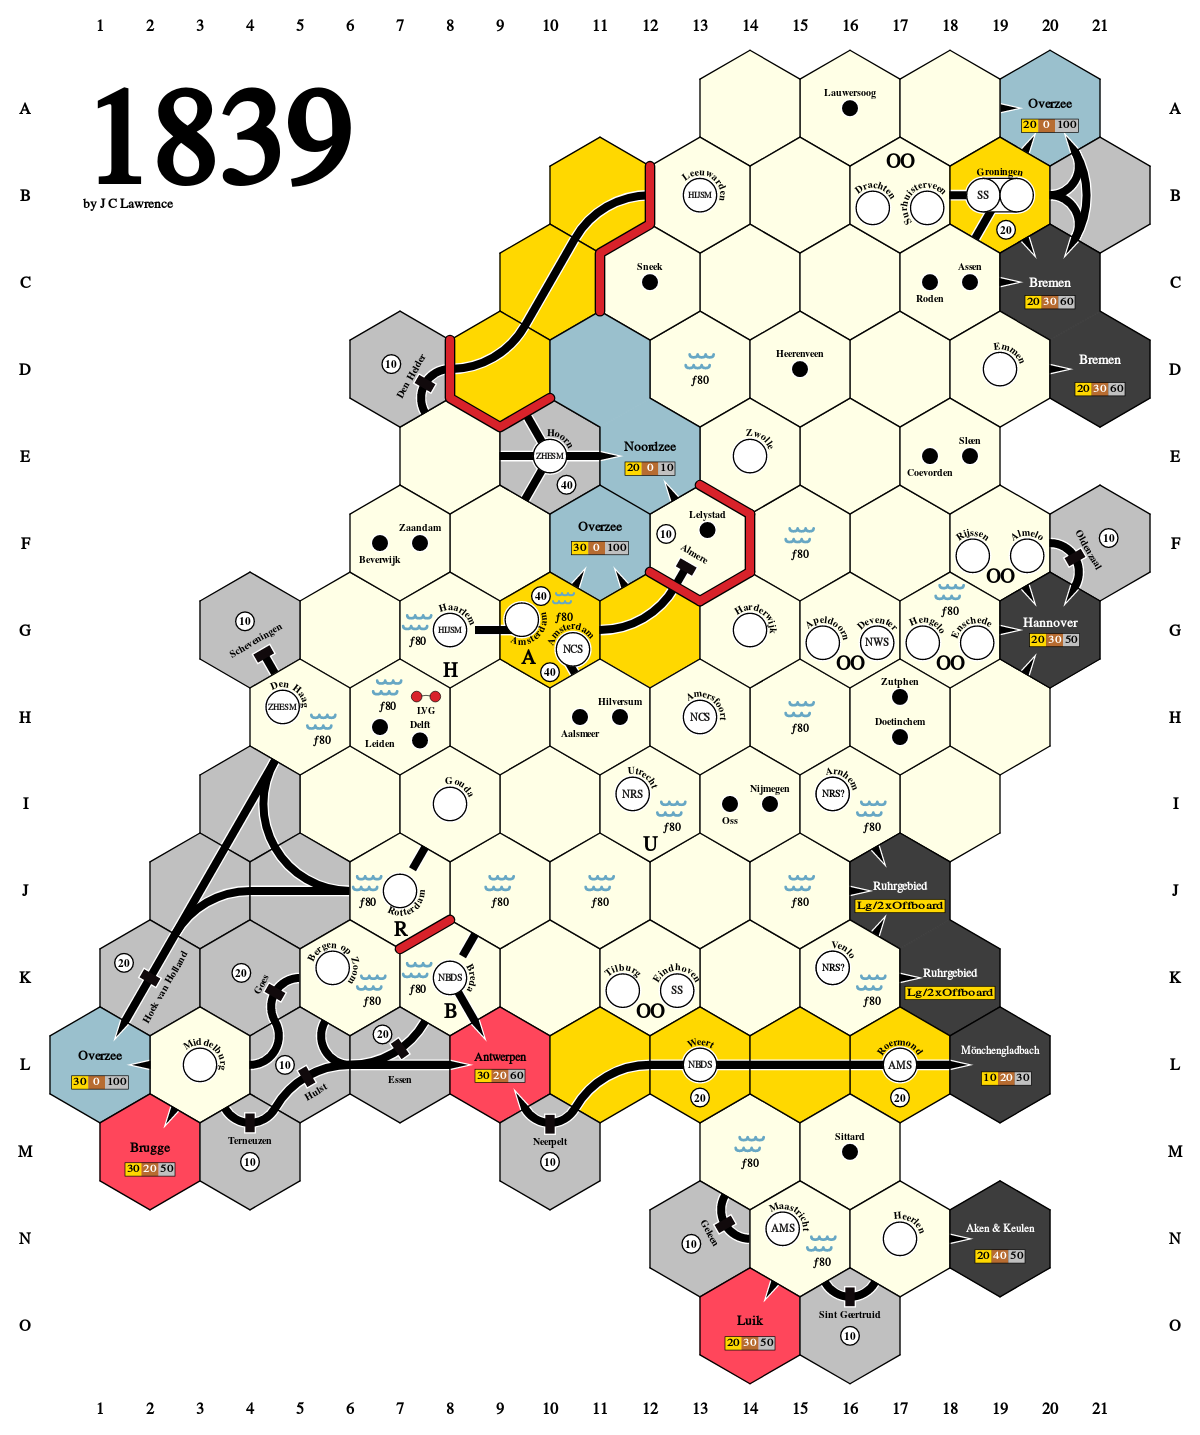
\includegraphics[width=6.75in,height=8.5in]{1839-Map}

\caption{1839 Game Map\label{fig:1828-Game-Map}}
\end{figure*}

\begin{itemize}
\item The map consists of hexagons of various types:
\begin{description}
\item [{Cities:}] City hexagons contain large circles along with the name(s)
of the cities.
\begin{description}
\item [{Big~Cities:}] Are marked with a letter (Amsterdam, Breda, Haarlem,
Rotterdam, Utrecht) and have a higher revenue.
\item [{OO~City:}] Have two distinct cities on the same tile and are marked
``OO'' but are otherwise the same as a normal city track tile. Only
OO city track tiles can be used on hexagons marked ``OO'', and they
cannot be used on any other map hexagons.
\end{description}
\item [{Towns:}] Town hexagons contain one or two small black circles marking
the towns for hexagons without track, or cross-bars on pre-built track.
\item [{Yellow~hexagons:}] Yellow hexagons represent yellow pre-built
track on the map. They can be upgraded using green track tiles in
green phase or later (see \secref{Game-Phases}).
\item [{Gray~hexagons:}] Gray hexagons contain pre-built track that may
not be altered nor upgraded. Track tiles cannot be placed on gray
hexagons, nor adjacent to them such that a line of track runs into
a blank gray hexagon-edge.
\item [{Off-board~locations:}] Black (Duitsland/Germany), blue (Overzees/Overseas),
and red (Belgie/Belgium) hexagons represent connections to areas not
shown on the map. Black triangles mark separate track connections
to those remote locations. Track tiles may be placed adjacent to them
so that the lines of track connect to the black triangles leading
to the remote connections. Track tiles cannot be placed adjacent to
an off-board hexagon such that a line of track runs into a blank off-board
hexagon-edge.
\item [{Rural~hexagons:}] All other hexagons are rural.
\end{description}
\item Terrain is marked with a wavy line (river) along with the terrain
cost for building track on those hexagons (always \textflorin 80).
\item Big cities have an upgrade cost (always \textflorin 80) that must
be plaid when upgrading a track tile on that hexagon.
\item Revenue centers and off-board locations are marked with their revenue
as a number in a small white circle, or as a series of numbers in
a coloured box matching the game phases at which they start applying
(see \tabref{Game-Phases} \& \subsecref{Run-train(s)}).
\item Some hexagons are marked with a red barbell, denoting that they are
blocked by a matching private company (see  \subsecref{Private-Companies}).
\item Some hexagon edges are blocked by dark brown barriers and track tiles
cannot be placed so as to make a new track connection across that
edge before dark brown phase (see \parref{track-placement-Overview}
\& \secref{Game-Phases}).
\item The Bremen (C20 \& D21) and Ruhrgebied (J17 \& K18) off-boards are
each a single location comprised of two hexagons.
\item Related terms:
\begin{description}
\item [{Revenue~center}] A city or town on a hexagon or track tile that
has an income or revenue value. Off-board hexagons are not revenue
centers.
\item [{Line~of~track}] A continuous track-connection between a hexagon
edge and a revenue center, or between a specific pair of hexagon edges
on the same or different hexagons.
\end{description}
\end{itemize}

\section{Stock Market\label{sec:Stock-Market}}

\begin{figure}
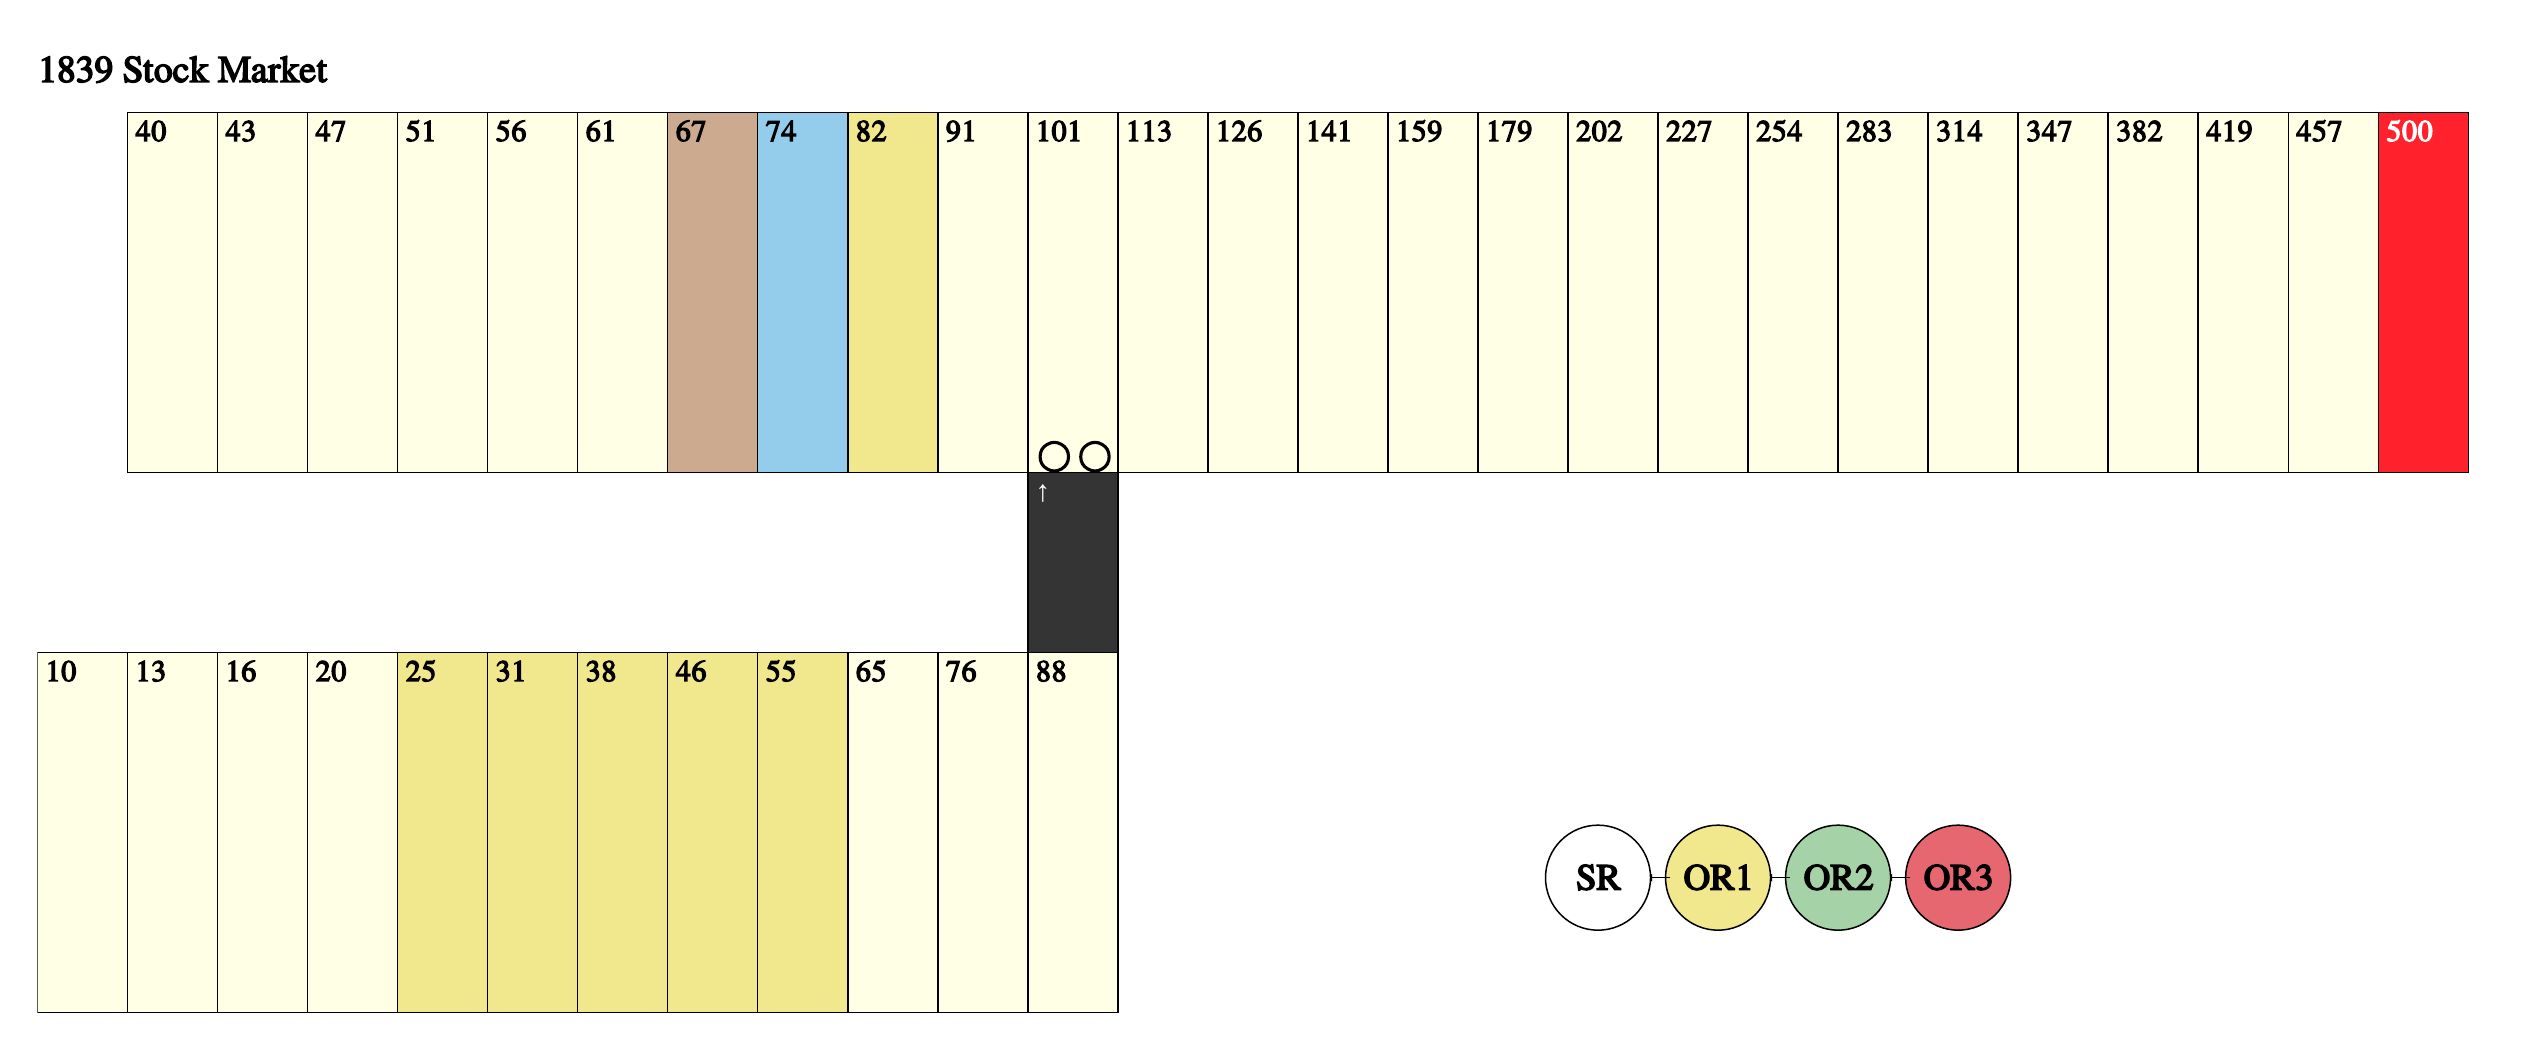
\includegraphics[angle=90,height=8.5in]{1839-Market}

\caption{Stock Market\label{fig:Stock-Market}}
\end{figure}


\subsection{Stock Market overview\label{subsec:Stock-Market-Overview}}
\begin{itemize}
\item Public companies have a stock price that is tracked on the Stock Market
with a stock price marker.
\item The Stock Market consists of two distinct markets:
\begin{itemize}
\item A Local Stock Market with values from \textflorin 10 to \textflorin 88
\item A Major Stock Market with values from \textflorin 40 to \textflorin 500.
\end{itemize}
\item The two markets join at \textflorin 101 on the Major Stock Market.
\begin{itemize}
\item Stock prices on the Major Stock Market cannot move onto the Local
Stock Market.
\item Stock prices on the Local Stock Market can move onto the Major Stock
Market.
\item A stock price on the Local Stock Market that moves right from \textflorin 88
moves to \textflorin 101 on the Major Stock Market or further right
as applicable (see \subsecref{Stock-price-movement}).
\item That company is now a Major Public Company and it and its assets are
subject to different rules (see ).
\end{itemize}
\item Public Companies with stock prices on the Local Stock Market are Local
Public Companies (see \subsecref{Public-Company-Overview}).
\item Public Companies with stock prices on the Major Stock Market are Major
Public Companies (see \subsecref{Public-Company-Overview})..
\item When a public company is parred, its stock price marker is placed
on the matching location on the Stock Market (see \subsecref{Starting-or-floating}).
\begin{itemize}
\item Both markets have an area of darker yellow (67/74/82 on the Major
Stock Market and 25/31/38/46/55 on the Local Stock Market) that mark
possible par prices for new public companies.
\end{itemize}
\item Both markets have large areas of pale-background spaces with no special
rules.
\item The \textflorin 500 price on the Major Stock Market has a red background.
The game ends if a stock price marker reaches \textflorin 500 (see
\subsecref{Game-end-criteria}).
\item Public company stock price markers move in well-defined ways (see
\subsecref{Stock-price-movement}).
\end{itemize}

\subsection{Stock price movement\label{subsec:Stock-price-movement}}
\begin{itemize}
\item The current stock price of a public company's shares is recorded on
a Stock Market with a stock price marker.
\item Stock price markers can move left or right along that Stock Market.
\begin{itemize}
\item If a stock price is to be moved left when it is already at the left
end of its Stock Market, it isn't moved.
\item If a stock price is to be moved right from \textflorin 88 on the Local
Stock Market, it is moved to \textflorin 101 on the Major Stock Market.
\begin{itemize}
\item If a stock price is to be moved right multiple times on the Local
Stock Market and passes \textflorin 88, then the stock price will
continue moving right the remaining number of times after the move
from \textflorin 88 to \textflorin 101 onto the Major Stock Market.
\end{itemize}
\item The game will end if a stock price marker reaches the largest price
on the Major Stock Market (\textflorin 500) (see \secref{Game-End}).
\end{itemize}
\item When a stock price marker is moved, it is placed under any stock price
markers already present in the new location.
\item For each 10\% share sold by a player, the stock price marker is moved
left once (see \subsecref{Selling-shares}).
\begin{itemize}
\item If shares of multiple companies are sold at the same time, the seller
must decide the order in which they are sold and thus the order in
which their stock price markers are moved and potentially the order
in which they will later operate (see \subsecref{Selling-shares}
\& \ref{subsec:company-operating-order}).
\end{itemize}
\begin{description}
\item [{Exception:}] Public companies can redeem their shares as they are
sold. In this case the stock price is not changed due to the sale.
(see \subsecref{Selling-shares}).
\end{description}
\item At the end of each Stock Round, the stock price markers of public
companies that have:
\begin{itemize}
\item One or more shares in the Bank Pool are moved left once (see \subsecref{company-operating-order}).
\item No shares left in both the IPO and Bank Pool are moved right once
(see \subsecref{company-operating-order}).
\end{itemize}
\item When a public company operates and pays or withholds a dividend, if
the total dividend paid is:
\begin{itemize}
\item Less than the current stock price, the stock price is moved left once
.
\item Zero because the company didn't have a train, then it is moved left
another time.
\item Equal to or larger than the current stock price, then the stock price
is moved right once.
\item Equal to or larger than double the current stock price, then the stock
price is moved right a second time.
\item (\emph{Local Public Companies only}) Equal to or larger than quadruple
the current stock price, then the stock price is moved right a third
time.
\item (\emph{Local Public Companies only}) Equal to or larger than octuple
the current stock price, then the stock price is moved right a fourth
time.
\end{itemize}
\end{itemize}

\section{Companies\label{sec:Companies}}

\subsection{Company types}
\begin{itemize}
\item There are two types of companies: private companies (see \subsecref{Private-Companies})
and public companies.
\item Private companies are represented by a single private company certificate,
may pay a revenue to their holder at the start of Operating Rounds,
and may grant their owner a special power, behaviour or benefit.
\item Public companies have shares that players may purchase and sell at
a share price that's tracked on one of the Stock Markets, and can
build track, place station markers, buy private companies and trains,
run trains, and pay or withhold dividends.
\end{itemize}

\subsection{Private companies\label{subsec:Private-Companies}}

\subsubsection{Private company general rules\label{subsec:Private-Companies-Overview}}
\begin{itemize}
\item Private companies pay their revenue from the bank to their owners
(a player or a public company) at the start of each Operating Round
(see \subsecref{Operating-round-General})\noun{.} Private companies
do not otherwise ``operate'' and do not lay track or buy or run
trains.
\item Private companies are discarded from the game when they close.
\item In green phase or later, public companies may purchase green private
companies from players (see \subsecref{Operating-round-actions})
at any time during the operation of the buying company (see \subsecref{Saleable-private-companies}).
\item In blue phase or later, public companies may purchase blue private
companies from players (see \subsecref{Operating-round-actions})
at any time during the operation of the buying company (see \subsecref{Saleable-private-companies}).
\item When a public company purchases a private company from a player:
\begin{itemize}
\item Both the director of the buying company and the owner of the private
company must agree to the purchase.
\item The purchase price may range from \textflorin 1 to the private company's
face value and is paid from the buying company's treasury to the selling
player.
\item Purchased private companies are moved to their owning company's charter
and future revenues from the private company will be paid to the owning
company's treasury.
\item The owning company may use the special power of the private company,
if any, when the owning company is operating from the point of purchase
onward and as long as the private company has not closed. Some private
company powers can only be used during certain steps of their owning
company's operations.
\end{itemize}
\item Brown private companies cannot be bought by public companies (see
\parref{Unsaleable-private-companies}).
\item Some private companies block specific hexagons on the map. Track tiles
cannot be built or upgraded at those hexagons by a public company
until the matching private company has been purchased by a public
company or closed.
\begin{itemize}
\item \noun{Het Laantje van der Gaag} blocks G19.
\item \noun{Rijkswaterstaat} blocks D10 and X57.
\end{itemize}
\item Private companies are discarded from the game when they close.
\end{itemize}

\subsubsection{Saleable private companies\label{subsec:Saleable-private-companies}}

\paragraph{Green private companies\label{par:Green-private-companies}}

\subparagraph{\noun{Het Laantje van der Gaag\label{par:Het-Laantje-van}}}
\begin{description}
\item [{Face~value:}] \textflorin 90
\item [{Revenue:}] \textflorin 10
\item [{Blocks:}] G19
\item [{Closes:}] When power used or the start of red phase.
\item [{Power:}] The owning public company may place an additional yellow
track tile (all terrain costs or upgrade costs must be paid) in addition
to the public company's normal track lay for \textflorin 20. If the
laid tile is at G19, then there is no terrain cost.
\item [{Use:}] Power may be used during the owning public company's track
build.
\end{description}

\subparagraph{\noun{Spoorlijn Roosendaal - Vlissingen\label{par:Spoorlijn-Roosendaal--}}}
\begin{description}
\item [{Face~value:}] \textflorin 100
\item [{Revenue:}] \textflorin 10
\item [{Blocks:}] None.
\item [{Closes:}] When power used or the start of red phase.
\item [{Power:}] Owning public company may place or upgrade a tile for
\textflorin 80 at Arnhem (K16) or Venlo (K18) as their yellow track
lay or upgrade respectively and may additionally place a station marker
in an empty and unreserved city location on that tile for free instead
of their normal station placement.
\item [{Use:}] Power may be used during the owning company's track build
and instead of the owning public company's station marker placement.
\end{description}

\paragraph{Blue private companies\label{par:Blue-private-companies}}

\subparagraph{\noun{Kabinet-Rochussen\label{par:Kabinet-Rochussen}}}
\begin{description}
\item [{Face~value:}] \textflorin 270
\item [{Revenue:}] \textflorin 20/\textflorin 0 (when owned by a public
company)
\item [{Blocks:}] None
\item [{Closes:}] When power used or the start of red phase.
\item [{Power:}] Owning public company may move one of its placed station
markets to a different location on the map for free. The new location
must be a legal station marker placement location for the company
before the move. A government station marker is placed at the prior
station marker location (see \subsecref{Government-railway}).\\
If the station marker is moved to a hexagon which already contains
one of the company's station markers, then the station marker already
on the hexagon is removed and a government station marker put in its
place (see \subsecref{Government-railway}).
\item [{Use:}] Instead of the owning public company's station market placement.
\end{description}

\subparagraph{\noun{Nederlandsche Fabriek van Werktuigen en Spoorwegmaterieel\label{par:Nederlandsche-Fabriek-van}}}
\begin{description}
\item [{Face~value:}] \textflorin 280
\item [{Revenue:}] \textflorin 0
\item [{Blocks:}] None.
\item [{Closes:}] At the start of red phase.
\item [{Power:}] Private company comes with three ``SAVED'' markers.
Other public companies may buy SAVED markets from the owning public
company, one per company per Operating Round, for \textflorin 150
each, paid to the treasury of the owning public company. The purchasing
company must immediately assign the bought SAVED marker to a train,
limit one per train. The owning company does not get a SAVED marker.\\
A train with a SAVED marker will discard its SAVED marker instead
of rusting, can be run in the next Operating Round, and will be discarded
from the game after its owning public company finishes operating in
the next Operating Round. Trains with a SAVED marker cannot be bought
between companies.
\item [{Use:}] N/A.
\end{description}

\subparagraph{\noun{Fabriek van Rijtuigen en Spoorwagens J. J. Beijnes\label{par:Fabriek-van-Rijtuigen}}}
\begin{description}
\item [{Face~value:}] \textflorin 290
\item [{Revenue:}] \textflorin 0
\item [{Blocks:}] None
\item [{Closes:}] At the start of light brown phase.
\item [{Power:}] Converts to a light brown train at the start of light
brown phase. The train is taken from the supply and the private company
is discarded from the game. If the private company is already owned
by a public company, the train is immediately placed in that public
company's treasury and may be run in the normal manner. If the private
company is owned by a player, the train is given to the player, may
be freely assigned to any company at any time, where-upon it can be
run and sold between public companies in the normal manner. Should
the train rust while still held by the player, there is no recompense.
\item [{Use:}] N/A.
\end{description}

\subparagraph{\noun{Cr�dit Mobilier\label{par:Cr=0000E9dit-Mobilier}}}
\begin{description}
\item [{Face~value:}] \textflorin 300
\item [{Revenue:}] \textflorin 30/\textflorin 0 (when owned by a public
company)
\item [{Blocks:}] None
\item [{Closes:}] At the start of red phase.
\item [{Power:}] When closed coverts to \textflorin 800 in cash taken from
the bank and a \noun{Rotterdamsche Bank} red private company, both
in the same location as this brown private company (see \subsecref{Red-private-companies}).\\
If owned by a public company when the public company is nationalised
(see \subsecref{Public-company-nationalisation}), then it is returned
to the director of the to-be-nationalised public company, along with
a \noun{Rotterdamsche Bank} red private company. The \noun{Cr�dit
Mobilier} can be repeatedly sold and returned in this way, each time
also giving a \noun{Rotterdamsche Bank} red private company to the
controlling player (see \subsecref{Red-private-companies}).
\item [{Use:}] In a 3-player game the\noun{ Cr�dit Mobilier} blue private
company is discarded from the game and not used (see \secref{Game-Setup}).
\end{description}

\subparagraph{\noun{Schielands Hoge Zeedijk\label{par:Schielands-Hoge-Zeedijk}}}
\begin{description}
\item [{Face~value:}] \textflorin 30
\item [{Revenue:}] \textflorin 30
\item [{Blocks:}] None.
\item [{Closes:}] At the start of red phase.
\item [{Power:}] Comes with two shares of the Founding Public Company associated
with the \noun{Rijkswaterstaat} brown private company during setup
(see \secref{Game-Setup}).
\item [{Use:}] N/A.
\end{description}

\subsubsection{Unsaleable private companies\label{par:Unsaleable-private-companies}}

\paragraph{Brown private companies\label{par:Brown-private-companies}}
\begin{itemize}
\item There are 5 brown private companies:
\begin{itemize}
\item \noun{August Borsig}
\item \noun{Cornelis Outshoorn}
\item \noun{Lodewijk Pincoffs}
\item \noun{Ketwich \& Voombergh}
\item \noun{Rijkwaterstaat}
\end{itemize}
\item In a 3-player game the \noun{Ketwich \& Voombergh} brown private company
is discarded from the game and not used (see \secref{Game-Setup}).
\item The unsaleable brown private companies are randomly assigned to founding
public companies during setup (see\secref{Game-Setup} \& \subsecref{Public-companies}).
\item Each of the unsaleable brown private companies has the following attributes:
\begin{description}
\item [{Face~value:}] \textflorin 280 (\textflorin 300 for the \noun{Rijkswaterstaat})
\item [{Revenue:}] \textflorin 30 (\textflorin 40 for the \noun{Rijkswaterstaat})
\item [{Blocks:}] None.
\item [{Closes:}] At the start of light brown phase or when the assigned
public company has acquired a train (see \tabref{Game-Phases} \&
\secref{Game-Phases}).
\item [{Power:}] When closed the owner of the brown private company may
take any single share of a parred company from the IPO.
\item [{Use:}] None.
\item [{Note:}] When purchased during the private auction comes with the
20\% director's certificate and a 10\% share certificate of the assigned
public company. The buying player must immediately set the par price
for the matching founding public company to any par price on the Major
Stock Market (see \secref{Stock-Market})\noun{. }An unsaleable brown
private company cannot be purchased by a public company.
\end{description}
\item In a 3-player game the \noun{Ketwich \& Voombergh} brown private company
is discarded from the game and not used (see \secref{Game-Setup}).
\end{itemize}
\newpage{}

\paragraph{Red private companies \label{subsec:Red-private-companies}}

\subparagraph{\noun{Rotterdamsche Bank\label{par:Rotterdamsche-Bank}}}
\begin{description}
\item [{Face~value:}] \textflorin 0
\item [{Revenue:}] \textflorin -100
\item [{Blocks:}] None.
\item [{Closes:}] Never.
\item [{Power:}] None.
\item [{Use:}] None.
\item [{Note:}] At the start of each Operating Round the owner of each
red private company must pay the red private company's revenue (\textflorin 100)
to the bank (see ).
\end{description}

\subsection{Public companies\label{subsec:Public-companies}}

\subsubsection{Public company overview \label{subsec:Public-Company-Overview}}

\begin{table*}
\begin{tabular}{>{\centering}p{5cm}c>{\centering}p{4cm}ccc}
\hline 
Name & Symbol & \multicolumn{2}{c}{Founding Public Company} & \multicolumn{2}{c}{Major Public Company}\tabularnewline
\cline{3-6} \cline{4-6} \cline{5-6} \cline{6-6} 
 &  & Homes & Stations & Homes & Stations\tabularnewline
\hline 
\hline 
\noun{Aken-Maastrichtsche Spoorweg-Maatschappij} & AMS & Roermond (L17), Maastricht (N15) & 5 & 2 & 5\tabularnewline
\hline 
\noun{Hollandsche IJzeren Spoorweg-Maatschappij} & HIJSM & Leeuwarden (B13), Haarlem (G8) & 4 & 2 & 5\tabularnewline
\hline 
\noun{Noord-Brabantsch-Duitsche Spoorweg-Maatschappi} & NBDS & Breda (K8), Weert (L13) & 4 & 2 & 5\tabularnewline
\hline 
\noun{Nederlandsche Centraal Spoorweg-Maatschappij} & NCS & Amsterdam (G11), Amersfoort (H13) & 3 & 2 & 5\tabularnewline
\hline 
\noun{Nederlandsche Rhijnspoorweg-Maatschappij} & NRS & Utrech (I12), choice of Arnhem (I16) or Venlo (K16) & 3 & 2 & 5\tabularnewline
\hline 
\noun{Nederlandsch-Westfaalsche Spoorweg-Maatschappij} & NWS & Deventer (G16) & 5 & 2 & 5\tabularnewline
\hline 
\noun{Maatschappij tot Exploitatie van Staatsspoorwegen} & SS & Groningen (B19), Eindhoven (K12) & 5 & 2 & 5\tabularnewline
\hline 
\noun{Zuid-Hollandsche Electrische Spoorweg-Maatschappij} & ZHESM & Hoorn (E10), Den Haag (H5) & 5 & 2 & 5\tabularnewline
\hline 
\noun{Spoorweg-Maatschappij \#1} & S1 &  &  & 2 & 5\tabularnewline
\hline 
\noun{Spoorweg-Maatschappij \#2} & S2 &  &  & 2 & 5\tabularnewline
\hline 
\noun{Spoorweg-Maatschappij \#3} & S3 &  &  & 2 & 5\tabularnewline
\hline 
\noun{Spoorweg-Maatschappij \#4} & S4 &  &  & 2 & 5\tabularnewline
\hline 
\noun{Spoorweg-Maatschappij \#5} & S5 &  &  & 2 & 5\tabularnewline
\hline 
\noun{Spoorweg-Maatschappij \#6} & S6 &  &  & 2 & 5\tabularnewline
\hline 
\noun{Spoorweg-Maatschappij \#7} & S7 &  &  & 2 & 5\tabularnewline
\hline 
\noun{Spoorweg-Maatschappij \#8} & S8 &  &  & 2 & 5\tabularnewline
\hline 
\end{tabular}

\caption{Public companies\label{tab:Public-Companies}}
\end{table*}

\begin{itemize}
\item There are sixteen public companies (see \tabref{Public-Companies}).
\item Each public company consists of:
\begin{itemize}
\item 9 share certificates:
\begin{itemize}
\item One 20\% director's certificate.
\item Eight 10\% certificates.
\end{itemize}
\item 5 station markers (see \tabref{Public-Companies})
\item A charter for holding and tracking the company treasury.
\item A stock price marker.
\end{itemize}
\item Public companies can be parred on the Local Stock Market or Major
Stock Market.
\begin{description}
\item [{Local~Public~Companies}] have stock prices on the Local Stock
Market.
\item [{Major~Public~Companies}] have stock prices on the Major Stock
Market.
\end{description}
\item Public companies once parred (see \subsecref{Starting-or-floating})
have a stock price, tracked on the stock market with a stock price
marker (see ).
\item The first eight listed public companies (ASM, HIJSM, NBDS, NCS, NRS,
NWS, SS, ZHESM) are Founding Public Companies. They:
\begin{itemize}
\item Have pre-defined home station location(s) (see \tabref{Public-Companies}).
\item Must be parred on the Major Stock Market as Major Public Companies
(see \secref{Stock-Market}) the first time they are parred.
\item Have varying numbers of home stations and place-able station markers
depending on the company (see \subsecref{Place-station-marker}).
\item After being nationalised (see \subsecref{Public-company-nationalisation}),
they:
\begin{itemize}
\item Can subsequently be parred as either Local or Major Public Companies
on the Local or Major Stock Market.
\item No longer have pre-defined home station locations (see \tabref{Public-Companies}).
\item Have 2 home stations and 3 place-able station markers.
\end{itemize}
\end{itemize}
\item The 8 numbered \noun{Spoorweg-Maatschappij} can be parred and floated
as either Local or Major Public Companies.
\item Public companies may:
\begin{itemize}
\item Buy green private companies (green phase or later, see \secref{Game-Phases}
\& \subsecref{Private-Companies}).
\item Buy blue private companies (blue phase or later, see \secref{Game-Phases}
\& \subsecref{Private-Companies}).
\item Place and upgrade track tiles (see \subsecref{Build-track} \& \subsecref{Track-placement-=000026-upgrades})
\item Place or swap station markers (see \subsecref{Place-station-marker}).
\item Buy and run trains (see \subsecref{Run-train(s)}, \subsecref{Buy-train(s)}
\& \secref{Trains-and-Running-Trains}).
\item Pay or withhold dividends (see \subsecref{Pay-or-withhold}).
\end{itemize}
\end{itemize}

\subsubsection{Public company directors\label{subsec:Company-directors}}
\begin{itemize}
\item The player that holds the most shares of a public company (largest
total percentage) is the director of the company, has the 20\% director's
share of the company and controls all of that company's operations
(if it has floated (see \subsecref{Starting-or-floating})).
\item The director's certificate can never be sold, only transferred to
another player. Once a company has floated, there is always a player
that owns the 20\% director's certificate and is the director of the
company until the company is nationalised or the game ends (see ).
\item If a player acquires shares such that they own a larger percentage
of the public company than the current director, they become the new
company director and exchange company certificates totaling 20\% of
the company for the 20\% director's certificate of the company, taking
control of the company charter and its assets.
\item In order to transfer director control of a company via share sales
or share donation (see \subsecref{Selling-shares} ):
\begin{itemize}
\item Another player must own at least 20\% of the company in order for
the exchange to take place.
\item The director's certificate must be exchanged for certificates of the
player with the most shares of the company after the sale or donation,
assigning control of the public company and its charter and assets
to that player.
\item The previous director must sell or donate sufficient shares of the
public company such that they own fewer shares of the public company
than the new director after the sale.
\begin{itemize}
\item In the case of a tie among other players for the most shares after
the sale or donation, the next tied player in player number card order
from the current director becomes the new director.
\end{itemize}
\end{itemize}
\end{itemize}

\subsubsection{Public company nationalisation\label{subsec:Public-company-nationalisation}}

\paragraph{Nationalisation overview\label{subsec:Nationalisation-overview}}
\begin{itemize}
\item When a public company buys the first train of a new rank that rusts
other trains, public companies may nationalise.
\item In operating order (see \subsecref{company-operating-order}) each
public company that still owns a currently unrusted train, including
the company that bought the rusting train, may nationalise.
\begin{itemize}
\item A rusted train marked with a SAVE token (see \parref{Nederlandsche-Fabriek-van})
does not qualify a public company to be able to nationalise.
\item A player that holds a brown train from the \noun{Fabriek van Rijtuigen
en Spoorwagens J. J. Beijnes} brown private company may assign it
to a public company at this time in order to qualify it for nationalisation
(see \parref{Fabriek-van-Rijtuigen}).
\end{itemize}
\end{itemize}

\paragraph{Nationalisation process\label{subsec:Nationalisation-process}}
\begin{enumerate}
\item Any cash in the company treasury is returned to the bank.
\item All shares of the company are returned from the players, company treasury,
Bank Pool, and IPO to the supply without recompense.
\item The company's station makers on the map are replaced by government
station markers (see \subsecref{Government-railway}).
\item All station markers and the stock price marker for the company are
returned to the supply.
\item All other assets (trains, private companies) held by the company are
discarded from the game without recompense.
\begin{description}
\item [{Exception:}] If the public company owned the \noun{Cr�dit Mobilier}
brown private company, then it and a \noun{Rotterdamsch Bank} red
private company certificate are given to the director of the company
being nationalised (see \parref{Cr=0000E9dit-Mobilier} \& \parref{Rotterdamsche-Bank}).
\end{description}
\item The company charter is returned to the supply.
\item If the nationalised company was a Founding Public Company, it is no
longer a Founding Public Company for the rest of the game (see pub\subsecref{Public-Company-Overview}).
\end{enumerate}

\subsection{Government railway\label{subsec:Government-railway}}
\begin{itemize}
\item The Government railway (\noun{Nederlandse Spoorwegen}) is represented
by a number of station markers.
\item Government station markers replace the station markers of:
\begin{itemize}
\item Nationalised public companies (see \subsecref{Nationalisation-process}).
\item The origin of moved station markers (see \parref{Kabinet-Rochussen}).
\item Station markers removed when a company acquires two station markers
in the same hexagon (see \parref{Kabinet-Rochussen}).
\end{itemize}
\item Newly parred public companies may choose government station marker
locations for their home stations.
\begin{itemize}
\item When the company operates and places its home stations, government
station markers can be replaced with the company's home stations (see
).
\end{itemize}
\item When placing a station marker during an Operating Round, public companies
may replace government station markers (that aren't reserved) with
their own station marker (see ).
\item Government station markers limit Major public company operations in
the same manner as other public company station markers (see ) and
do not limit Local Public Company operations (see ).
\end{itemize}

\section{Track Tiles\label{sec:Track}}

\subsection{Track tiles overview\label{subsec:Track-Tile-Overview}}
\begin{itemize}
\item There are yellow, green and brown track tiles.
\item Track tiles are limited to those available in the supply.
\item At the beginning of the game only yellow track tiles are available.
\item Yellow track tiles are placed directly on rural and city hexagons
of the map.
\item Green track tiles upgrade/replace yellow track tiles and yellow map
hexagons.
\item Brown track tiles upgrade/replace green track tiles.
\item Gray track tiles upgrade/replace brown track tiles.
\item Upgraded track tiles are returned to the supply for later use.
\end{itemize}

\subsection{Track types\label{subsec:Track-types}}
\begin{itemize}
\item Outside of colour, there are three types of track tiles:
\begin{description}
\item [{City}] Have one or more white circles for station markers and a
revenue value (number in a small white circle). Only city track tiles
can be used on city map hexagons, and they cannot be used on any other
map hexagons. 
\begin{description}
\item [{Big~City:}] Are marked with a letter (``A'', ``B'', ``H'',
``R'' or ``U'' for Amsterdam, Breda, Haarlem, Rotterdam and Utrecht)
and have a higher revenue. Only matching city track tiles can be used
on those cities and they cannot be used on any other map hexagons. 
\item [{OO~City:}] Have two distinct cities on the same tile and are marked
``OO'' but are otherwise the same as a normal city track tile. Only
OO city track tiles can be used on hexagons marked ``OO'', and they
cannot be used on any other map hexagons.
\end{description}
\item [{Town:}] Have a small cross-bar marking the town with a line of
track passing through it, and a revenue value (number in a small white
circle). Only town track tiles may be placed on town map hexagons,
and they cannot be used on any other map hexagons. 
\begin{description}
\item [{Double~town:}] Have two distinct track lines, each of which has
a small cross-bar marking the separate towns. Only double town track
tiles may be placed on such map hexagons, and they cannot be used
on any other map hexagons.
\end{description}
\item [{Plain}] Have one to four lines of track without towns or cities,
that directly connect pairs of edges of the hexagon. Plain track tiles
can be used on rural map hexagons, and cannot be used on any other
map hexagons.
\end{description}
\end{itemize}

\subsection{Track placement \& upgrades \label{subsec:Track-placement-=000026-upgrades}}

\subsubsection{Track placement overview \label{par:track-placement-Overview}}
\begin{itemize}
\item Only yellow track tiles are available at the beginning of the game.
Later in the game green, brown and finally gray track tiles become
available (see \tabref{Game-Phases} \& \subsecref{Upgrading-track}).
\item Track tiles can be placed on the towns, cities and rural hexagons
of the map and cannot be placed on off-board hexagons or gray pre-built
hexagons (see \secref{Map-Explanation}).
\item After placing or upgrading a track tile the placing public company
must be able to trace a continuous line of track from one of its station
markers to a line of track on the placed track tile without:
\begin{itemize}
\item Passing through a city with all of station-marker spaces filled with
other public company's station markers or (for Major Public Companies
) government station markers.
\item Crossing any hexagon-edge twice.
\end{itemize}
\item Track tiles must not be placed such that a line of track:
\begin{itemize}
\item Already present is not preserved by the new track tile. (Only the
connectivity is important, not the exact shape of the line of track)
\item Runs off the edge of the map (no further hexagons).
\item Runs to the edge of a gray pre-built hexagon that doesn't have pre-printed
track running to it.
\item Runs to the edge of an off-board hexagon that doesn't have a black
triangle/arrow to indicate a continuation for the track.
\item Makes a new track connection across a dark brown barrier before dark
brown phase (see \secref{Map-Explanation}).
\end{itemize}
\item A company placing a track tile on a water terrain (\textflorin 80)
hexagon that has not previously contained a track tile must pay the
terrain cost from its treasury to the bank before placing the tile
(see \secref{Map-Explanation}).
\begin{itemize}
\item Once a track tile of a given type is placed in a hexagon, terrain
costs for the hexagon are not paid again in future tile upgrades.
\begin{description}
\item [{Exception:}] The big cities (Amsterdam, Breda, Haarlem, Rotterdam,
Utrecht) have an \textflorin 80 upgrade fee for each upgrade.
\end{description}
\end{itemize}
\end{itemize}

\subsubsection{Upgrading track\label{subsec:Upgrading-track}}
\begin{itemize}
\item Starting in green phase:
\begin{itemize}
\item public companies may upgrade yellow track tiles and yellow map hexagons
to green track tiles (see \tabref{Game-Phases}).
\end{itemize}
\item Starting in brown phase:
\begin{itemize}
\item public companies may also upgrade green track tiles to brown track
tiles (see \tabref{Game-Phases}).
\end{itemize}
\item When upgrading a track tile:
\begin{itemize}
\item The type of the track tile cannot be changed.
\item Connections of pairs of hexagon edges by lines of track must be preserved.
\item Connections of city circles to hexagon edges by lines of track must
be preserved.
\item A public company cannot upgrade a track tile it has previously upgraded
or placed in that same Operating Round.
\end{itemize}
\item The upgraded track tile is returned to the supply for future use.
\item Once a track tile on a river or hill hexagon is upgraded, the terrain
cost is not paid again (see \secref{Map-Explanation}).
\begin{description}
\item [{Exception:}] The big cities (Amsterdam, Breda, Haarlem, Rotterdam,
Utrecht) have an \textflorin 80 upgrade fee for each upgrade.
\end{description}
\item Station markers are moved to their corresponding locations on the
new tile when upgrading a track tile or hexagon.
\end{itemize}

\section{Trains \& Running Trains\label{sec:Trains-and-Running-Trains}}

\subsection{Trains overview\label{subsec:Trains-Overview}}
\begin{itemize}
\item Public companies run and buy trains during Operating Rounds (see \subsecref{Run-train(s)}
and \subsecref{Buy-train(s)}).
\item Public companies run trains on ``routes'' to generate revenue (see
\subsecref{Run-train(s)}).
\item Different types of trains have different restrictions for their routes
(see \subsecref{Route-definitions-by-train-type}).
\item Local public companies have different restrictions for their routes
than major public companies (see \subsecref{Public-Company-Overview}
\& \subsecref{Public-Company-Overview}).
\item Cities' and towns' revenues can be counted towards a company's revenue
only once, no matter how many of the company's trains include the
city or town in their route.
\begin{description}
\item [{Exception:}] ``R'' trains can count the revenue of a city or
town toward company revenue that a different train run by the same
company has already counted.
\end{description}
\item The number of trains a public company can own is controlled by the
train limit (see \subsecref{Train-Limit}).
\item Public companies with a route from one of their station markers to
another revenue center (an off-board is insufficient) must own at
least one train at the end of their turn in an Operating Round (see
offboards \& \subsecref{General-Route-definition} \& \subsecref{Emergency-train-buying})
\item Trains are available from the supply in colour order:
\begin{itemize}
\item First yellow, then green, blue, light brown, dark brown, red, gray
and finally purple.
\item All the trains of a given colour must be bought from the supply before
the trains of the next colour are available (see \subsecref{Buy-train(s)}
\& \tabref{Game-Phases}).
\end{itemize}
\item Trains are purchased one at a time with any phase changes occurring
before the company purchases any more trains in that Operating Round.
\item The purchase of trains of new types causes phase changes and may change
the train limit (see \tabref{Game-Phases} \& \subsecref{Train-Limit}).
\end{itemize}

\subsection{Route definition \label{subsec:General-Route-definition}}
\begin{itemize}
\item A route is a single continuous line of track that:
\begin{itemize}
\item Contains at least two revenue centers (town or city, not off-board)
(see \secref{Map-Explanation}).
\item Can begin or end at a town, city or off-board.
\begin{itemize}
\item Local Public Companies cannot include off-boards in their routes;
Major Public Companies can.
\item Off-boards at the ends of Major Public Company routes add to the total
company revenue (once per train-route that includes them) but do not
require train length to include them in the route.
\end{itemize}
\item Must pass through a city containing one of the owning public company's
station makers.
\item Can pass through a city with an open station marker location.
\item (\emph{Local Public Companies only}) Can pass through a city containing
a government station marker location.
\item Can include separate revenue centers on the same hexagon (see \subsecref{Track-types}).
\item Can use multiple entirely separate lines of track on the same tile.
\begin{description}
\item [{Note:}] Track tiles such as \#16, \#19, \#20 etc and parts of \#43,
\#44, \#45 \& \#46 etc represent railway bridges and thus lines of
track that do not intersect.
\end{description}
\item Can enter a city from one direction and exit in any other connected
direction.
\end{itemize}
\item Additionally, a route cannot:
\begin{itemize}
\item Cross the same hexagon-edge more than once.
\item Use the same piece of track on a track tile more than once (no matter
how small the track section may be).
\item Pass through a city that doesn't have an open station marker location
and doesn't contain the public company's station marker and (Local
Public Companies only) doesn't contain a Government station marker.
\item Run to or through the same revenue center more than once.
\item Have both ends of the route in an off-board of the same colour (black,
blue or red).
\end{itemize}
\item The routes of multiple trains run by the same public company during
an Operating Round cannot share or re-use any line of track.
\begin{itemize}
\item The routes can meet or cross at provided that they use entirely separate
sections of track.
\end{itemize}
\item Off-board triangle connections are termini. Routes may not run into
an off-board location via one black triangle and proceed back onto
the board via another.
\end{itemize}

\subsection{Running trains by train-type \label{subsec:Route-definitions-by-train-type}}

\subsubsection{``L'' trains\label{subsec:L-trains}}
\begin{itemize}
\item Cannot be bought from the supply.
\item Cannot be bought between companies.
\item Can only be owned by Local Public Companies.
\item Until dark brown phase, an ``L'' train of is given to Local Public
Companies from the supply at the start of their first Operating Round:
yellow in yellow phase, green in green phase, and blue in blue and
light brown phases (see ).
\item If a Local Public Company become a Major Public Company, any L-train
it owns is returned to the supply.
\end{itemize}

\subsubsection{``R'' trains\label{subsec:R-trains}}
\begin{itemize}
\item ``R'' trains can count cities and towns on their routes for revenue
that other trains in the same company have already included in their
routes.
\item Any red trains that have already run in an Operating Round are removed
at the start of purple phase.
\item Red trains that have not yet run in an Operating Round are removed
immediately after they do run in an Operating Round.
\item Red trains cannot be bought between public companies in purple phase.
\end{itemize}

\subsubsection{\emph{N}~trains \label{subsec:Ntrains}}
\begin{itemize}
\item The route for an \emph{N} train (where \emph{N} is 2, 4 or 7) cannot
contain more than a total of \emph{N} revenue centers, where \emph{N}
is the number on the train card.
\begin{description}
\item [{Revenue:}] The sum of all the revenue centers on the route whose
revenues are not included in the routes of other trains owned by the
company plus (Major Public Companies only) any off-boards of different
colours at the ends of the routes.
\begin{description}
\item [{Exception:}] The routes for ``R'' trains can include revenue
centers that are included in the routes of other trains owned by the
company.
\end{description}
\end{description}
\end{itemize}

\subsubsection{2+1 trains \label{subsec:2+1-trains}}
\begin{itemize}
\item The route for a\emph{ 2+1} train cannot contain more than a total
of \emph{3} revenue centers, no more than two of which are cities.
\begin{description}
\item [{Revenue:}] The sum of all the revenue centers on the route that
are not included in the routes of other trains owned by the company
\end{description}
\end{itemize}

\subsubsection{N+ trains \label{subsec:N+-trains}}
\begin{itemize}
\item The route for a N+ train cannot contain more than a total of N cities.
There may be any number of towns on the route; before, between and
after any other revenue centers on the route.
\begin{description}
\item [{Revenue:}] The sum of all the revenue centers on the route whose
revenues are not included in the routes of other trains owned by the
company plus (Major Public Companies only) any off-boards of different
colours at the ends of the routes.
\begin{description}
\item [{Exception:}] The routes for ``R'' trains can include revenue
centers that are included in the routes of other trains owned by the
company.
\end{description}
\end{description}
\end{itemize}

\subsubsection{Diesel trains \label{subsec:Dieseltrains}}
\begin{itemize}
\item The route for a Diesel train may contain an unlimited number of revenue
centers.
\begin{description}
\item [{Revenue:}] The sum of all the revenue centers on the route whose
revenues are not included in the routes of other trains owned by the
company plus (Major Public Companies only) any off-boards of different
colours at the ends of the routes.
\begin{description}
\item [{Exception:}] The routes for ``R'' trains can include revenue
centers that are included in the routes of other trains owned by the
company.
\end{description}
\end{description}
\end{itemize}

\subsection{Train limit\label{subsec:Train-Limit}}
\begin{itemize}
\item The number of trains a public company can own is limited by the game
phase (see \parref{Train-purchasing} \& \secref{Game-Phases} \&
\subsecref{Systems}). A public company can own trains up to the current
train limit.
\item A public company that has not reached its train limit may buy trains
that would cause it to exceed the train limit after the game phase
change caused by the purchase takes effect.
\item Train limits are checked and enforced on all public companies as each
trains is bought.
\begin{itemize}
\item A public company with more trains than the current train limit must
discard its trains from the game until it is within the current train
limit.
\end{itemize}
\end{itemize}

\section{Game Phases \label{sec:Game-Phases}}

\subsection{Yellow phase}
\begin{itemize}
\item The game begins in yellow phase.
\item Yellow track tiles are available.
\item Yellow trains are available.
\item Train limit is 4.
\item There is 1 Operating Round per set after Stock Rounds.
\end{itemize}

\subsection{Green phase}
\begin{itemize}
\item Green phase starts with the purchase of the first green train.
\item Green private companies may be bought by public companies.
\item Green and yellow track tiles are available.
\item Train limit is 4.
\item There are 2 Operating Rounds per set after Stock Rounds.
\end{itemize}

\subsection{Blue phase}
\begin{itemize}
\item Blue phase starts with the purchase of the first blue train.
\item Blue private companies may be bought by public companies.
\item Green and yellow track tiles are available.
\item All yellow trains are removed from the game.
\item Companies with a green or blue train can nationalise.
\item Train limit is 4.
\item There are 2 Operating Rounds per set after Stock Rounds.
\end{itemize}

\subsection{Light brown phase}
\begin{itemize}
\item Brown phase starts with the purchase of the first brown train.
\item Private companies may be bought by public companies.
\item Brown, green and yellow track tiles are available.
\item Revenue centers with multiple values use the second (brown) value.
\item All green trains are removed from the game.
\item Companies with a blue or light brown train can nationalise.
\item Train limit is 3.
\item There are 3 Operating Rounds per set after Stock Rounds.
\end{itemize}

\subsection{Dark brown phase}
\begin{itemize}
\item Brown phase starts with the purchase of the first brown train.
\item Private companies may be bought by public companies.
\item Brown, green and yellow track tiles are available.
\item Revenue centers with multiple values use the second (brown) value.
\item All blue trains are removed from the game.
\item Companies with a light brown or far brown train can nationalise.
\item Train limit is 3.
\item There are 3 Operating Rounds per set after Stock Rounds.
\end{itemize}

\subsection{Red phase}
\begin{itemize}
\item Red phase starts with the purchase of the first red train.
\item All private companies close.
\item Brown, green and yellow track tiles are available.
\item Revenue centers with multiple values use the second (brown) value.
\item All light brown trains are removed from the game.
\item Companies with a dark brown or red train can nationalise.
\item Train limit is 3.
\item There are 3 Operating Rounds per set after Stock Rounds.
\end{itemize}

\subsection{Gray phase}
\begin{itemize}
\item Gray phase starts with the purchase of the first gray train.
\item Gray, brown, green and yellow track tiles are available.
\item Revenue centers with multiple values use the second (brown) value.
\item All dark brown trains are removed from the game.
\item Companies with a red or gray train can nationalise.
\item Train limit is 2.
\item There are 3 Operating Rounds per set after Stock Rounds.
\end{itemize}

\subsection{Purple phase}
\begin{itemize}
\item Purple phase starts with the purchase of the first purple train.
\item Gray, brown, green and yellow track tiles are available.
\item Revenue centers with multiple values use the second brown value.
\item All red trains are removed from the game.
\item Companies with a gray or purple train can nationalise.
\item Train limit is 2.
\item There are 4 Operating Rounds per set after the Stock Round.
\item The game ends after the first set of Operating Rounds in purple phase.
\end{itemize}

\end{document}
